\documentclass[11pt]{article}
\usepackage[a4paper,margin=1in]{geometry}
\usepackage{amsmath,amssymb,amsthm}
\usepackage{tikz}
\usepackage{xcolor}
\usepackage[hidelinks]{hyperref}
\hypersetup{pdftitle={Cycles of length 2^n - 2 in the de Bruijn graph},pdfauthor={Vamshi Jandhyala}}
\setlength{\parskip}{0.4em}
\setlength{\parindent}{0pt}

\newtheorem{theorem}{Theorem}
\newtheorem{lemma}{Lemma}
\theoremstyle{remark}
\newtheorem*{remark}{Remark}

\definecolor{inkblue}{RGB}{40,76,105}
\definecolor{softblue}{RGB}{226,235,243}
\definecolor{rust}{RGB}{153,70,45}

\title{Cycles of length $2^n-2$ in the binary de Bruijn graph}
\author{Vamshi Jandhyala}
\date{}

\begin{document}
\maketitle
\vspace{-2em}

\begin{abstract}
The binary de Bruijn graph $B(n)$ has $2^{2^{n-1}-n}$ cycles through all of its $2^n$ vertices. A count of
the cycles that miss exactly two vertices, attributed to Kibler in 1972, appears in a 1982 survey with only an
outline of a proof, and the formula printed there gives $4$ for $n=3$, where there are $3$. We prove that the number is
$\tfrac13\bigl(2^n-(-1)^n\bigr)\,2^{2^{n-1}-2n+2}$. The two missing vertices are either $0^n$ and $1^n$ or the
two alternating strings. The first case is the de Bruijn count; in the second, the Laplacian changes by a
matrix of rank one, and the determinant can be evaluated exactly because a random walk on the de Bruijn graph
is uniform after $n-1$ steps. Evaluated at $n-1$, the printed expression is the count of the second case. The algebra
is checked in the Lean proof assistant.
\end{abstract}

\section{The question}

Write $0$s and $1$s around a circle so that every block of three consecutive symbols is different. With eight
symbols every one of the eight blocks of length three appears once; there are two such circles, $00010111$
and $00011101$, read cyclically. Now allow six symbols. How many circles are there? Stop and try this before
reading on.

There are three: $000111$, $001011$ and $001101$. The first misses the blocks $010$ and $101$; the other two
are the circles of length eight with one $0$ and one $1$ removed from their runs of three, so they miss $000$
and $111$.

In graph terms, the vertices of the de Bruijn graph $B(n)$ are the binary strings of length $n$, with an edge
from $a_1a_2\cdots a_n$ to $a_2\cdots a_nb$ for $b\in\{0,1\}$. A cycle of length $L$ in $B(n)$ is the same as
a circle of $L$ symbols in which every block of $n$ consecutive symbols occurs at most once. For $L=2^n$ these
are the de Bruijn cycles, and Flye Sainte-Marie~\cite{FSM} and de Bruijn~\cite{dB46} found that there are
$2^{2^{n-1}-n}$ of them (de Bruijn's note~\cite{dB75} records the priority).

In 2016 Timothy Chow asked on MathOverflow~\cite{MO} about a count of the cycles of length $2^n-2$ that
Fredricksen's survey of shift-register cycles~\cite[Section~2c]{F82} attributes to Kibler (personal
communication, 1972). The survey gives only an outline: the BEST theorem reduces the count to a determinant,
which ``by induction'' can be evaluated, and the total is printed as
$\tfrac13\,2^{2^n-2n}\bigl(2^{n-1}+(-1)^n\bigr)$~\cite[p.~203]{F82}, which is $4$ for $n=3$. Chow's
question quotes it correctly; the slip is in the survey.

\begin{theorem}\label{thm:main}
For $n\ge2$ the de Bruijn graph $B(n)$ has
\[
T(n)=\frac{2^n-(-1)^n}{3}\;2^{\,2^{n-1}-2n+2}
\]
cycles of length $2^n-2$. Of these, $2^{2^{n-1}-n}$ miss the vertices $0^n$ and $1^n$, and
\[
\tfrac13\bigl(2^{n-2}-(-1)^n\bigr)\,2^{2^{n-1}-2n+2}
\]
miss the two alternating strings $0101\cdots$ and $1010\cdots$.
\end{theorem}

The first factor of $T(n)$ is the Jacobsthal number $1,3,5,11,21,\dots$ and the second a power of two; the
values for $n=2,3,4,5,6$ are $1,3,20,2816,88080384$. The count of the second kind is the printed expression
evaluated at $n-1$.

\section{Two edges left out}

Put $m=n-1$. A string of length $n$ is an edge of $B(m)$, from its first $m$ symbols to its last $m$, so the
vertices of $B(n)$ are the edges of $B(m)$ and a cycle in $B(n)$ is a closed walk in $B(m)$ that uses no edge
twice. A cycle of length $2^n-2$ uses every edge of $B(m)$ except two; call the two unused edges $R$. The
cycle is then an Eulerian circuit of $B(m)-R$.

Every vertex of $B(m)$ has two edges in and two out, and an Eulerian graph has as many edges in as out at
every vertex, so the two edges of $R$ also enter and leave each vertex equally often. Two edges with that property form either two loops or a cycle of
length two.

\begin{lemma}\label{lem:two}
The loops of $B(m)$ are at $0^m$ and $1^m$, and its only cycle of length two joins the alternating strings
$p=\cdots0101$ and $q=\cdots1010$.
\end{lemma}

\begin{proof}
A loop at $u$ means that shifting $u$ by one place gives $u$ back, so all its symbols are equal. If $u\to v\to
u$ with $u\ne v$, shifting $u$ by two places gives $u$ back, so $u$ has period two and is not constant.
\end{proof}

\begin{figure}[ht]
\centering
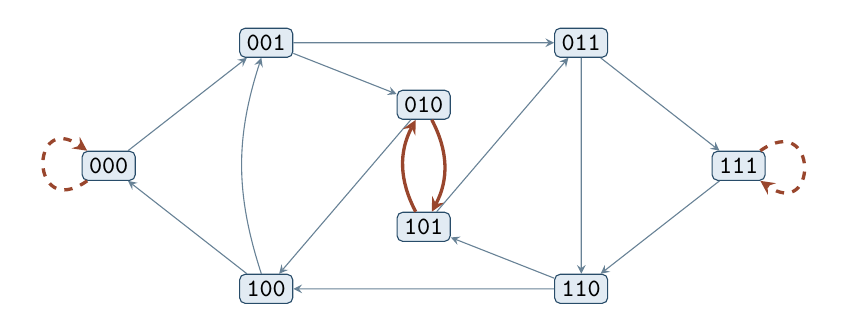
\begin{tikzpicture}[>=stealth, scale=1.25, every node/.style={font=\small},
  vtx/.style={draw=inkblue, fill=softblue, rounded corners=2pt, inner sep=2.5pt, font=\ttfamily\small}]
\node[vtx] (000) at (0,0) {000};
\node[vtx] (001) at (1.6,1.25) {001};
\node[vtx] (100) at (1.6,-1.25) {100};
\node[vtx] (010) at (3.2,0.62) {010};
\node[vtx] (101) at (3.2,-0.62) {101};
\node[vtx] (011) at (4.8,1.25) {011};
\node[vtx] (110) at (4.8,-1.25) {110};
\node[vtx] (111) at (6.4,0) {111};
\draw[->, rust, very thick, dashed] (000) to[out=215, in=145, looseness=6] (000);
\draw[->, inkblue!70] (000) to[] (001);
\draw[->, inkblue!70] (001) to[] (010);
\draw[->, inkblue!70] (001) to[] (011);
\draw[->, inkblue!70] (100) to[] (000);
\draw[->, inkblue!70] (100) to[bend left=18] (001);
\draw[->, inkblue!70] (010) to[] (100);
\draw[->, rust, very thick] (010) to[bend left=28] (101);
\draw[->, rust, very thick] (101) to[bend left=28] (010);
\draw[->, inkblue!70] (101) to[] (011);
\draw[->, inkblue!70] (011) to[] (110);
\draw[->, inkblue!70] (011) to[] (111);
\draw[->, inkblue!70] (110) to[] (100);
\draw[->, inkblue!70] (110) to[] (101);
\draw[->, inkblue!70] (111) to[] (110);
\draw[->, rust, very thick, dashed] (111) to[out=35, in=-35, looseness=6] (111);
\end{tikzpicture}

\caption{The de Bruijn graph $B(3)$. A cycle of length $14$ in $B(4)$ is an Eulerian circuit of $B(3)$ with
two edges removed: the two dashed loops (case A) or the two thick edges between $010$ and $101$ (case B).}
\label{fig:b3}
\end{figure}

By the BEST theorem~\cite{AEdB51,ST41}, the number of Eulerian circuits of a connected graph with in-degree
equal to out-degree everywhere is the number of spanning arborescences rooted at any vertex $w$, times
$\prod_v(d^+(v)-1)!$. Here every out-degree is $1$ or $2$, so the product is $1$ and each case counts
arborescences. (If $B(m)-R$ is disconnected it has no arborescence and no Eulerian circuit, so the count is
still right; this happens only in case B with $m=1$.)

\paragraph{Case A.} A loop is never part of an arborescence, so deleting the loops changes nothing and case A
gives the de Bruijn number $2^{2^m-m-1}=2^{2^{n-1}-n}$. Directly: delete the two loop steps from a de Bruijn
cycle.

\section{The alternating case}

Here is the route. Tutte's matrix-tree theorem~\cite{T48} turns the number of arborescences into a determinant
of the Laplacian. Deleting the two edges of the cycle $p\leftrightarrow q$ changes the Laplacian by a matrix of
rank one, so by the matrix determinant lemma the ratio of the two tree counts is $1-w^{\mathsf T}Gw$ for one
vector $w$ and a matrix $G$ that inverts the Laplacian. That inverse is a finite sum, because a random walk on
$B(m)$ forgets where it started after exactly $m$ steps.

Let $N=2^m$, let $P$ be the transition matrix of the walk that shifts in a uniformly random bit, and let $J$
be the all-ones matrix. The Laplacian of $B(m)$ is $L=2(I-P)$ (loops cancel). Deleting $p\to q$ and $q\to p$
lowers the out-degrees of $p$ and $q$ by one and removes the two entries, so the new Laplacian is
\[
L' = L - e_p(e_p-e_q)^{\mathsf T} - e_q(e_q-e_p)^{\mathsf T} = L - ww^{\mathsf T},\qquad w=e_p-e_q .
\]

\begin{lemma}\label{lem:cof}
If a matrix $M$ has zero row sums and zero column sums, all its cofactors are equal to one number $c(M)$, and
$\det(M+J)=N^2c(M)$.
\end{lemma}

\begin{proof}
If $M$ has rank $N-2$ or less, every cofactor and $\det(M+J)$ vanish. Otherwise its kernel and left kernel are
both spanned by $\mathbf 1$, and $M\operatorname{adj}(M)=\operatorname{adj}(M)M=0$ forces
$\operatorname{adj}(M)=cJ$. The matrix determinant lemma in the form $\det(M+uv^{\mathsf T})=\det M+v^{\mathsf
T}\operatorname{adj}(M)u$, with $u=v=\mathbf 1$, gives $\det(M+J)=0+c\,\mathbf 1^{\mathsf T}J\mathbf 1=N^2c$.
\end{proof}

By the matrix-tree theorem the number of arborescences of each graph is the cofactor of its Laplacian, so the
ratio we want is $\det(L'+J)/\det(L+J)$.

\begin{lemma}[exact mixing]\label{lem:mix}
$P^m=J/N$. For $0\le k<m$, $P^k(u,v)=2^{-k}$ if $v$ is $u$ shifted by $k$ places (with any $k$ new symbols),
and $0$ otherwise.
\end{lemma}

\begin{proof}
After $k$ steps the last $k$ symbols are uniform random and the rest are $u$ shifted; after $m$ steps nothing
of $u$ is left.
\end{proof}

Put $Z=\sum_{k=0}^{m-1}(P^k-J/N)$. Since $PJ=J$, the sum telescopes: $(I-P)Z=I-P^m=I-J/N$. Also
$Z\mathbf 1=0$ and $\mathbf 1^{\mathsf T}Z=0$, because $P$ has row and column sums $1$. For $y=\tfrac12Zw$ this
gives $(L+J)y=(I-J/N)w+J\,\tfrac12Zw=w$, using $\mathbf 1^{\mathsf T}w=0$. So $y$ is the solution we need, and
\[
\det(L+J-ww^{\mathsf T}) = \det\bigl((L+J)(I-yw^{\mathsf T})\bigr) = \det(L+J)\,\bigl(1-w^{\mathsf T}y\bigr).
\]
In words: deleting the 2-cycle multiplies the tree count by $1-w^{\mathsf T}y$, and $w^{\mathsf T}y$ is half
the sum of the numbers $w^{\mathsf T}P^kw$ over $k<m$.

Each of those is a statement about returning. The strings $p$ and $q$ have period two, so shifting $p$ by an
even number of places can give $p$ back and never $q$, and an odd shift does the opposite
(Figure~\ref{fig:shift}). By Lemma~\ref{lem:mix},
\[
w^{\mathsf T}P^kw = P^k(p,p)+P^k(q,q)-P^k(p,q)-P^k(q,p) = 2\left(-\tfrac12\right)^k \qquad(0\le k<m),
\]
and therefore
\[
1-w^{\mathsf T}y = 1-\sum_{k=0}^{m-1}\left(-\tfrac12\right)^k = \frac{2^{m-1}+(-1)^m}{3\cdot2^{m-1}} .
\]
Multiplying by the de Bruijn number $2^{2^m-m-1}$ gives case B,
$\tfrac13\,2^{2^m-2m}\bigl(2^{m-1}+(-1)^m\bigr)$, which with $m=n-1$ is the formula in
Theorem~\ref{thm:main}. Adding case A,
\[
2^{2^{n-1}-2n+2}\left(2^{n-2}+\frac{2^{n-2}-(-1)^n}{3}\right) = \frac{2^n-(-1)^n}{3}\,2^{2^{n-1}-2n+2}=T(n). \qquad\square
\]

\begin{figure}[ht]
\centering
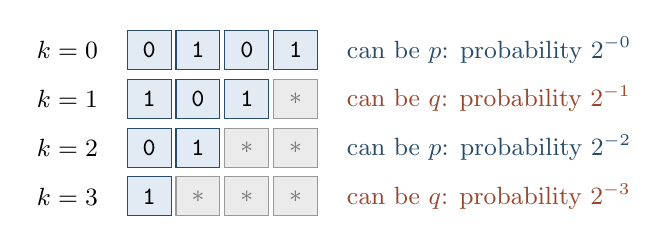
\begin{tikzpicture}[x=0.62cm, y=0.62cm, every node/.style={font=\small}]
\node[anchor=east] at (-0.4,0) {$k=0$};
\draw[fill=softblue, draw=inkblue] (0,-0.4) rectangle (0.9,0.4);
\node[font=\ttfamily\small] at (0.45,0) {0};
\draw[fill=softblue, draw=inkblue] (1,-0.4) rectangle (1.9,0.4);
\node[font=\ttfamily\small] at (1.45,0) {1};
\draw[fill=softblue, draw=inkblue] (2,-0.4) rectangle (2.9,0.4);
\node[font=\ttfamily\small] at (2.45,0) {0};
\draw[fill=softblue, draw=inkblue] (3,-0.4) rectangle (3.9,0.4);
\node[font=\ttfamily\small] at (3.45,0) {1};
\node[anchor=west, text=inkblue] at (4.3,0) {can be $p$: probability $2^{-0}$};
\node[anchor=east] at (-0.4,-1) {$k=1$};
\draw[fill=softblue, draw=inkblue] (0,-1.4) rectangle (0.9,-0.6);
\node[font=\ttfamily\small] at (0.45,-1) {1};
\draw[fill=softblue, draw=inkblue] (1,-1.4) rectangle (1.9,-0.6);
\node[font=\ttfamily\small] at (1.45,-1) {0};
\draw[fill=softblue, draw=inkblue] (2,-1.4) rectangle (2.9,-0.6);
\node[font=\ttfamily\small] at (2.45,-1) {1};
\draw[fill=black!8, draw=black!40] (3,-1.4) rectangle (3.9,-0.6);
\node[text=black!55] at (3.45,-1) {$\ast$};
\node[anchor=west, text=rust] at (4.3,-1) {can be $q$: probability $2^{-1}$};
\node[anchor=east] at (-0.4,-2) {$k=2$};
\draw[fill=softblue, draw=inkblue] (0,-2.4) rectangle (0.9,-1.6);
\node[font=\ttfamily\small] at (0.45,-2) {0};
\draw[fill=softblue, draw=inkblue] (1,-2.4) rectangle (1.9,-1.6);
\node[font=\ttfamily\small] at (1.45,-2) {1};
\draw[fill=black!8, draw=black!40] (2,-2.4) rectangle (2.9,-1.6);
\node[text=black!55] at (2.45,-2) {$\ast$};
\draw[fill=black!8, draw=black!40] (3,-2.4) rectangle (3.9,-1.6);
\node[text=black!55] at (3.45,-2) {$\ast$};
\node[anchor=west, text=inkblue] at (4.3,-2) {can be $p$: probability $2^{-2}$};
\node[anchor=east] at (-0.4,-3) {$k=3$};
\draw[fill=softblue, draw=inkblue] (0,-3.4) rectangle (0.9,-2.6);
\node[font=\ttfamily\small] at (0.45,-3) {1};
\draw[fill=black!8, draw=black!40] (1,-3.4) rectangle (1.9,-2.6);
\node[text=black!55] at (1.45,-3) {$\ast$};
\draw[fill=black!8, draw=black!40] (2,-3.4) rectangle (2.9,-2.6);
\node[text=black!55] at (2.45,-3) {$\ast$};
\draw[fill=black!8, draw=black!40] (3,-3.4) rectangle (3.9,-2.6);
\node[text=black!55] at (3.45,-3) {$\ast$};
\node[anchor=west, text=rust] at (4.3,-3) {can be $q$: probability $2^{-3}$};
\end{tikzpicture}

\caption{The walk started at $p=0101$ ($m=4$). After $k$ steps the state is $p$ shifted by $k$ places (blue)
followed by $k$ random bits ($\ast$). For even $k$ the blue part is how $p$ starts, so the walk is at $p$ with
probability $2^{-k}$ and never at $q$; for odd $k$ it is how $q$ starts. By symmetry the same holds from $q$,
which gives $w^{\mathsf T}P^kw=2(-\frac12)^k$.}
\label{fig:shift}
\end{figure}

\begin{remark}
The factor $(2^{m-1}+(-1)^m)/(3\cdot2^{m-1})$ tends to $\tfrac13$: in the limit, a third of the arborescences
avoid both edges of the 2-cycle. Göttfert~\cite{G06} studies the minimal polynomials of binary sequences of
least period $2^N-2$; we found no count of the cycles of length $2^n-2$ in the literature we could reach.
\end{remark}

\paragraph{Verification.} The counts $1,3,20,2816$ for $n\le5$ agree with a direct enumeration of cycles, and
both cases agree with exact determinants for $n\le11$, in two programs that share no code. Lemma~\ref{lem:two}
(in the form: the only two-edge sets whose deletion keeps $B(m)$ balanced are the two loops and the alternating
2-cycle), the effect of each deletion on the Laplacian, Lemma~\ref{lem:mix}, the identity $(I-P)Z=I-J/N$, the
solution $y$, the determinant identity, the evaluation of $w^{\mathsf T}P^kw$ and the closed forms are checked in
Lean~4 with Mathlib~\cite{mathlib}, using only the standard axioms. The BEST theorem, the matrix-tree theorem,
Lemma~\ref{lem:cof} and the de Bruijn count are cited, not formalised. Everything is at
\url{https://github.com/jvvk/mathematics/tree/main/debruijn-cycles-two-short}.

\paragraph{Acknowledgements.} The question was asked by Timothy Chow on MathOverflow, and the comment there by
Steve Huntsman pointed to the matrix determinant lemma. Anthropic's Claude (Opus~5.5) was used to find the
argument, write the programs and the Lean formalisation, and draft this text. The author takes responsibility
for the content.

\begin{thebibliography}{9}
\bibitem{AEdB51} T.~van Aardenne-Ehrenfest and N.~G.~de Bruijn, Circuits and trees in oriented linear graphs,
\emph{Simon Stevin} \textbf{28} (1951) 203--217; reprinted in \emph{Classic Papers in Combinatorics},
Birkh\"auser, 149--163, \href{https://doi.org/10.1007/978-0-8176-4842-8_12}{doi:10.1007/978-0-8176-4842-8\_12}.
\bibitem{dB46} N.~G.~de Bruijn, A combinatorial problem, \emph{Nederl. Akad. Wetensch. Proc.} \textbf{49}
(1946) 758--764.
\bibitem{dB75} N.~G.~de Bruijn, Acknowledgement of priority to C.~Flye Sainte-Marie on the counting of circular
arrangements of $2^n$ zeros and ones that show each $n$-letter word exactly once, T.H.-Report 75-WSK-06,
Technological University Eindhoven (1975).
\bibitem{FSM} C.~Flye Sainte-Marie, Solution to question nr.~48, \emph{l'Interm\'ediaire des
Math\'ematiciens} \textbf{1} (1894) 107--110.
\bibitem{F82} H.~Fredricksen, A survey of full length nonlinear shift register cycle algorithms, \emph{SIAM
Rev.} \textbf{24} (1982) 195--221, \href{https://doi.org/10.1137/1024041}{doi:10.1137/1024041}; open copy at
\url{https://hdl.handle.net/10945/61146}.
\bibitem{G06} R.~G\"ottfert, Sequences of period $2^N-2$, in \emph{Sequences and Their Applications, SETA 2006},
Lecture Notes in Comput. Sci. \textbf{4086}, Springer (2006) 223--236,
\href{https://doi.org/10.1007/11863854_19}{doi:10.1007/11863854\_19}.
\bibitem{MO} T.~Chow, Cycles of length $2^n-2$ in the de Bruijn graph, MathOverflow question 227666
(4 January 2016), \url{https://mathoverflow.net/q/227666}, accessed 11 October 2026.
\bibitem{ST41} C.~A.~B.~Smith and W.~T.~Tutte, On unicursal paths in a network of degree 4, \emph{Amer. Math.
Monthly} \textbf{48} (1941) 233--237,
\href{https://doi.org/10.1080/00029890.1941.11991103}{doi:10.1080/00029890.1941.11991103}.
\bibitem{T48} W.~T.~Tutte, The dissection of equilateral triangles into equilateral triangles, \emph{Proc.
Cambridge Philos. Soc.} \textbf{44} (1948) 463--482,
\href{https://doi.org/10.1017/S030500410002449X}{doi:10.1017/S030500410002449X}.
\bibitem{mathlib} The mathlib Community, The Lean mathematical library, in \emph{Proceedings of the 9th ACM
SIGPLAN International Conference on Certified Programs and Proofs (CPP 2020)}, 367--381,
\href{https://doi.org/10.1145/3372885.3373824}{doi:10.1145/3372885.3373824}.
\end{thebibliography}

\bigskip
\noindent Vamshi Jandhyala, London, UK.

\end{document}
